\chapter{Toolchain Implementation - Frontend}\label{chap:offline}
The purpose of the toolchain is to support the proposed model from specifying assertions for Smart Contracts, transforming them to their negation to generating assertion Smart Contracts that can be invoked by the validators. As determined in \secref{sec:restrict}, the current version of the toolchain only supports the processing of assertions featuring universal quantification. The toolchain was developed in the programming language OCaml \cite{ocaml_docs} --- the code is available in a GitHub\footnote{\url{https://github.com/proglang/thesis-distributed-assertion-checking}\todo{commit}} repository of the Chair of Programming Languages.

As an overview, \figref{fig:pipeline_frontend} depicts all stages of the processing pipeline implemented by the toolchain. The colourized stages highlight the frontend, which was designed to be as generic as possible, s.t. it can be used (or extended) to support any target blockchain. For the target-specific processing, the intermediate result of the frontend is passed to the respective backends via a public interface.

\begin{figure}[h]
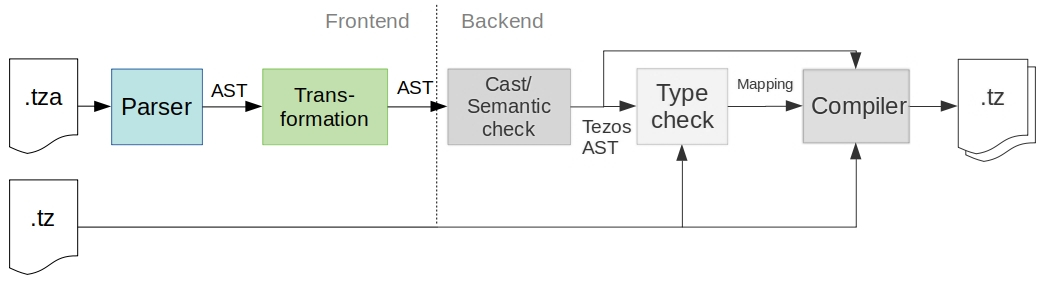
\includegraphics[width=\linewidth]{figures/3-offline/pipeline_frontend}
\caption{The stages of the generic frontend of the compilation pipeline}
\label{fig:pipeline_frontend}
\end{figure}

First, developers can specify assertions in a domain-specific language, which is described in \secref{sec:syntax}. The toolchain then parses the assertions into abstract syntax trees (ASTs), which are passed to the transformation stage. In this stage, the ASTs are transformed into ASTs that represent their negation. This is described further in \secref{sec:transformation}. The resulting ASTs are then passed to the backend, which is introduced in the subsequent chapter for the Tezos blockchain.
%Lastly, \secref{sec:accuracy} analyses the reliability of distributed assertion checking as proposed and to what extent it affects the costs.

\section{Assertion syntax}\label{sec:syntax}
Tezos' Smart Contract language Michelson is a low-level and stack-based language. Specifying assertions that way is complex and inconvenient, especially if the language is compiled to other targets as well. Therefore, this thesis defines a domain-specific high-level language to express assertions. 

The syntax of this language is described in two versions by the EBNF grammars given in appendix \ref{apx:grammar}. One version implements a prefix and the other one an infix notation. The parser currently supports the prefix notation and correct operator precedences must be handled explicitly with parentheses. To avoid context switches (for developers on Tezos), the syntax is inspired by OCaml \cite{ocaml_docs} and uses the same type notations as Michelson.

\subsection{Code structure}
Assertions are passed to the toolchain as simple text files. This thesis follows the convention of using the file extension \texttt{.tza} for such files (henceforth referred to as ``assertion contracts'') in reference to the file extension \texttt{.tz}used for Michelson source files. Assertion contracts contain at least one assertion for a specific entrypoint of the actual contract (henceforth referred to as ``parent contract''). For the remaining entrypoints the compiler automatically generates empty assertions\footnote{cf. \secref{sec:compiler}}.

An assertion begins with the keyword \texttt{entrypoint} and a signature consisting of an optional tag denoted by \%, followed by a parameter pattern. Parameter patterns are similar to patterns in OCaml --- they are templates that match shapes of data structures and bind identifiers to the components of them. The given parameter pattern must match exactly the parameter type of the entrypoint it is associated with. The body of an assertion can contain a nesting of quantifiers and conditions around exactly one \texttt{assert} expression. Conditions can be used to restrict the quantification domains or for any other constraints. For completeness, the existential quantifier is already included in the grammar, however the current version of the pipeline will reject any assertions containing it. 

How the assertions are associated with the respective entrypoint of the parent contract depends on the Smart Contract language. In the case of Solidity, a tag that mirrors the function name is enough to link assertion and entrypoint. In Michelson contracts, on the other hand, entrypoints can be anonymous. Therefore, the assertions are linked to the entrypoints through the tags, the parameter type or both. \secref{sec:typecheck} describes in more detail how the linking is implemented in the Tezos backend.

\subsection{Parameter patterns}
\lstref{lst:patterns} gives an overview of the parameter patterns supported in the assertion language.
\lstinputlisting[caption=Patterns in the assertion language, language=, numbers=none, label=lst:patterns]{listings/patterns.txt}

By using patterns, developers can avoid the explicit handling of special cases, such as empty lists, in the assertion specification. Furthermore, they can be used to put emphasis on the relevant components of the input parameters by replacing the irrelevant ones with wildcards. As an example, the assertion given in \lstref{lst:patterns_usage} concerns the left element of a pair and only applies to non-empty lists. 
\begin{lstlisting}[label=lst:patterns_usage, language=Assertion, numbers=none]
(entrypoint %g (pair (cons a as) _)  ...)
\end{lstlisting}

\subsection{Types and operations}
In order to make the frontend generic, the sets of data types and operations supported by the grammar constitute unions of those present in the target languages. This not only the implementation of a single, common parser, but also allows the transformation to be oblivious of the target platform. As a consequence, the backends are responsible for performing a semantic check and  rejecting any assertions containing types or operations which are not supported by the target language.

The current version of the language contains all data types present in Tezos' VM and a subset of operations that Michelson provides (as of protocol version 007 Delphi). Besides the primitive types \texttt{int}, \texttt{nat} (natural numbers), \texttt{string}, \texttt{bool}, \texttt{bytes} and \texttt{unit}, this includes composite types like \texttt{list}, \texttt{pair}, \texttt{map} or the union type \texttt{or}. Domain specific data types, like \texttt{timestamp} or \texttt{address}, are supported as well. The data type \texttt{fmu} represents a generic fractional monetary unit, which is translated to the corresponding token type of the target platform\footnote{Mutez in Tezos, or Wei in Ethereum}.

The grammar currently includes common arithmetic (e.g., \texttt{add}, \texttt{sub}, \texttt{abs}, \texttt{mod}), relational  (e.g., \texttt{eq}, \texttt{neq}, \texttt{lt}) and logic and bitwise operators (e.g., \texttt{and}, \texttt{or}, \texttt{lsr}, \texttt{lsl}). Some operations that operate on data structures (e.g., \texttt{nth} and \texttt{size}) are supported as well. Domain specific operations have not been included yet, but they may be added to the language if necessary. 

\subsection{Example}
The example given in \lstref{lst:sorted_assertion} implements an assertion, which checks whether a list is sorted in ascending order based on a variation of the formula stated in \eqref{eq:sorted} in the introduction:
\begin{equation}\label{eq:sorted_v2}
	(\forall n,m : int) (0 \leq n < m < |a|) \Rightarrow a[n] \leq a[m]
\end{equation}
In contrast to the previous variation, which translates to an assertion that compares a random element of the list with its direct neighbour, this translates to a comparison of two random elements (under the constraint $n < m$). \lstref{lst:sorted_assertion} shows how this formula can be expressed in the assertion language.
\lstinputlisting[caption=Assertion contract for checking if a list is sorted, language=Assertion, label={lst:sorted_assertion}]{listings/sorted.tza}

In line 1, the signature of the assertion is declared with tag \textit{find} and a parameter \texttt{a} of type integer list. The body is a nesting of two universal quantifiers which declare the predicate variables $n$ and $m$ of type integer (lines 2 and 3), followed by a nesting of conditions to define the domains of the quantifiers (lines 4-6), corresponding to the premise of the formula. The body of the last condition (line 7) ultimately contains the keyword \texttt{assert} followed by the specification of the property to be checked, i.e.,  $a[n] \leq a[m]$.

\subsection{Extensions}\label{sec:ext}
In future iterations, the assertion syntax could be extended with some more features to improve usability and readability:
\begin{itemize}
\item \textbf{Local variables} to store, reuse and denominate computed values
\item \textbf{User-defined functions} to extract whole routines that can be reused in a single or even many assertion contracts, if defined as a module.
\item \textbf{if-else conditions} to adapt the domains of quantifications if certain conditions hold. The assertion that checks whether two numbers are relatively prime (discussed in \secref{sec:coprime}) is a good use-case for this feature: Firstly, the minimum of the given number has to be determined, however the \texttt{min}-function might not be supported as a built-in function by the target language (Tezos, for instance, does not support it). A solution for that could be to implement two branches in the program to handle each case. Secondly, if the greater of the two numbers is not evenly divided by the smaller one, the formula can be optimized by reducing the quantification domain by half to $(2 \le n \le \lfloor \frac{min(a,b)}{2} \rfloor)$, as a number cannot be evenly divided by any number between itself and its half \cite{bernhardt_veigel_2020}. With a syntax supporting an \texttt{if-else} control structure, the optimized assertion could look as follows:
\lstinputlisting[caption=Assertion syntax with if-else structures \cite{bernhardt_veigel_2020}, language=Assertion, label={lst:coprime}]{listings/coprime_ifelse.tza}
This feature is not included in the current version, because conditional domain restrictions make the translation from quantifiers to random generators or loops more complex. Aside from that, without the feature of variables and user-defined functions, the code is inflated significantly, thus causing increased origination cost.
\end{itemize}

\section{Parser}
Assertions expressed in the syntax described above are passed as a simple text file to the pipeline. It is not admissible to generate empty assertions for all entrypoints of the parent contract, hence empty files are rejected. Furthermore, the parser guarantees total success or total failure of parsing the assertion by aborting execution immediately after encountering a syntax error. 

After successfully parsing all assertions, the parser returns a list of ASTs. On the toplevel, the AST type given in \lstref{lst:ast_type} is composed of an entrypoint specification and an assertion body. The parameter pattern and assertion body, in turn, are  subtrees representing their composition or the content of the assertion respectively.
\begin{lstlisting}[label=lst:ast_type, language=, numbers=none, caption=Toplevel AST type definition in OCaml]
type ast =
  {entrypoint : string option * pattern; body : assertion}
\end{lstlisting}

\figref{fig:ast_example} shows the resulting AST after parsing the assertion given in \lstref{lst:sorted_assertion}. The subtype representing quantifiers contains a special field \textit{Bounds}, which is initially left empty by the parser. During the transformation, it is populated with a set of constraints concerning its predicate variable, cf. \secref{sec:transformation}.

\section{Transformation}\label{sec:transformation}
The assertion, as specified by a developer, is modified in two ways before the compiler translates it into target code: firstly, it has to be transformed into its negation. Secondly, quantifiers are converted to random generators, which generate values within a specified range (corresponding to the domains of discourse). In the assertion language, the ranges can be expressed using \texttt{if}-conditions. As a preliminary for the compilation, the transformation additionally analyses the condition nodes of the AST, identifies conditions that state a range constraint for a generator and assigns it to the respective quantification node (by adding it to the \textit{Bounds} field). Therefore, the transformation contains two consecutive steps:
\begin{enumerate}
\itemsep-0.5em
\item Negation
\item Domain constraint analysis and assignment
\end{enumerate}
Each step is described in more detail in the following subsections.

\subsection{Negation}
The formula is negated according to the negation rules of second-order predicate logic and by applying De Morgan's laws \cite{de_morgan} until the negation is applied to the literals. Negating universal quantification is equivalent to an existential quantification of its negated body (and vice versa): $\neg \forall x P(x) \equiv \exists x \neg P(x)$ \cite{Sundstrom2020Quantifiers}. The domain restrictions are not affected by the negation, which is also reflected in the rules of predicate logic if the domain is given as a premise in the logical formula: $\neg (p \Rightarrow q) \equiv p \Rightarrow \neg q $.

Applied to an AST representation of the assertion, the negation recursively traverses the \texttt{assertion} subtree, replaces quantifier and expression nodes with the corresponding negations and skips condition nodes. The output is thus a modified AST. 
Further pursuing the example of the assertion for sorted lists, the negated version of the AST given in \figref{fig:ast_example} is shown in \figref{fig:ast_example_neg}. The universal quantifiers have been transformed to existential quantifiers, and the asserted condition from $a[n] <= a[m]$ to $a[n] > a[m]$.

\begin{figure}[t]
\hfill
\subfloat[AST after parsing\label{fig:ast_example}]{%
  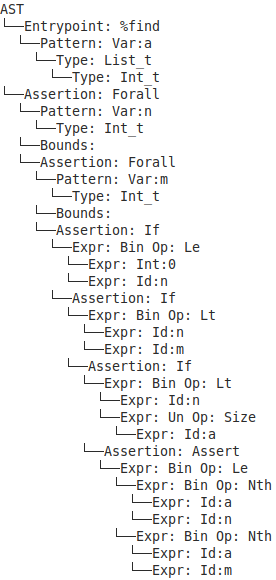
\includegraphics[width=0.33\textwidth]{figures/3-offline/ast_example_find}
}
\subfloat[Negated AST\label{fig:ast_example_neg}]{%
  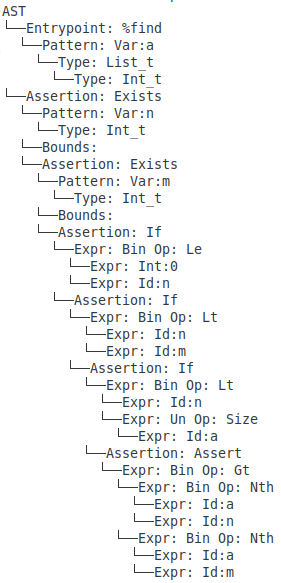
\includegraphics[width=0.33\textwidth]{figures/3-offline/ast_example_neg}
}
\hfill
\subfloat[Fully transformed AST\label{fig:ast_example_transf}]{%
  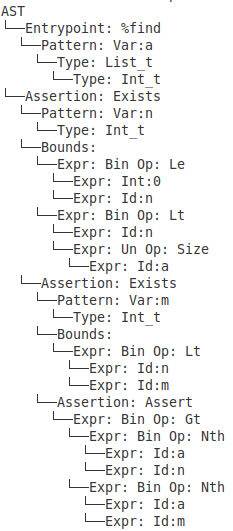
\includegraphics[width=0.3\textwidth]{figures/3-offline/ast_example_transf}
}
\caption{Modifications to the sorted list assertion AST from parsing to completed transformation}
\end{figure}

\subsection{Domain assignment}
In order to obtain random generators which only generate values in the interesting range, i.e., within the domains of discourse, the second step of the transformation skims the condition nodes of the AST for atomic constraints that contain bound variables. These conditions are then moved to the \texttt{Bounds} field of the respective quantifier. If the constraint contains more than one bound variable, it is assigned to the quantifier with the highest depth in the quantifier nesting, as they depend on the generated values of the previous generators. \\
Relating to the example of sorted lists, the premise in \eqref{eq:sorted_v2} can be considered as a conjunction of the four constraints
\begin{enumerate}
\itemsep-1em
\item $0 \leq n$
\item $n < |a| $
\item $n \le m$ and
\item $m < |a|$.
\end{enumerate}
Constraint 1,2 and 4 only contain one bound variable ($n$ or $m$), thus they are assigned to the respective quantifier binding it. Constraint 3, on the other hand, features two bound variables -- this constraint is assigned to the quantifier last in the nesting, thus the quantifier binding $m$. The corresponding AST expressing this assignment is shown in \figref{fig:ast_example_transf}. 

During compilation, the quantifiers, and their list of bounds, are then translated to target code that corresponds to the following pseudocode (\lstref{lst:rand}):
\begin{lstlisting}[label=lst:rand, caption=Random generators for sorted list assertion, numbers=none]
n = random(0, size(a))
m = random(n + 1, size(a))
\end{lstlisting}

However, if constraints contain certain operators, deriving efficient random generators is less straight-forward. Consider the following constraints:
\begin{enumerate}
\itemsep-0.7em
\item $(\forall n : int) (n < 10 \lor n > 20) ...$
\item $(\forall n : int) (n \ne 10) ...$
\item $(\forall n : int) (n = 10) ...$
\end{enumerate}
Constraint 1 can complicate restricting the range of the random generator in two ways. Firstly, it separates the range into two disjoint sub-ranges, which translates to a random generator as shown in \lstref{lst:rand_disjoint}.
\begin{lstlisting}[label=lst:rand_disjoint, caption=Random generator with two disjoint ranges, numbers=none]
n = if random(0,2) == 0 then random(-MAX_INT, 10)
                        else random(21, MAX_INT)
\end{lstlisting}
Secondly, the operands of a disjunction cannot be considered separately if they involve several bound variables. For the predicate variable whose random generator is executed first, the domain restriction is optional, while the generation of the following random values depend on the previous result. \lstref{lst:rand_disjoint_nm} shows the corresponding random generators for a variation of constraint 1 featuring two bound variables, i.e., $(\forall n,m) (n < 10 \lor m > 20)...$.
\begin{lstlisting}[label=lst:rand_disjoint_nm, caption=Random generators with two disjoint ranges and two bound variables, numbers=none]
n = if random(0,2) == 0 then random(-MAX_INT, 10)
                        else random(-MAX_INT, MAX_INT)
m = if n < 10 then random(-MAX_INT, MAX_INT)
              else random(20, MAX_INT)
\end{lstlisting}
Similarly to 1, constraint 2 splits the domain into sub-domains. Constraint 3 effectively makes the quantifier binding $n$ obsolete and thus can be translated to a variable with a constant value.

In the current implementation of the transformation, constraints featuring the logical or, exclusive or or inequality operator are kept as part of the assertion body. They are considered to be exceptional cases, but will increase the overall complexity of the compilation beyond the scope of a first iteration. In the case that constraints remain part of the assertion body, they are checked during runtime. As a consequence, an invocation of the assertion contract can result in a futile assertion check if such a condition is not met.

\subsubsection{Implicit constraints}
In some cases, boundaries are imposed to the random generators implicitly through the used data types. List indices, for instance, are always bound to the range $0.. size(list) - 1$ and could thus be derived from the formula without an explicit specification. As this requires a semantic analysis of the AST and thus a more complex transformation, the current implementation requires a completely explicit formula in terms of the domains. 

Depending on the blockchain VM, the lower bound for generated values used in indexing operations can be implicitly handled by the random generator of an appropriate predicate variable type. As an example, Michelson supports the data type \texttt{nat} representing the natural numbers, which categorically excludes all values below zero. \eqref{eq:sorted_v2} can thus be abbreviated with the formula given in \eqref{eq:sorted_v2_abbr}.
\begin{equation}\label{eq:sorted_v2_abbr}
	(\forall n : nat)(\forall m : nat) (n \le m < |a|) \Rightarrow a[n] \leq a[m]
\end{equation}

\section{Accuracy of the approach}\label{sec:accuracy}
\todo{Idea: own chapter "probabilistic model" oder so - OR: model description}
Since the proposed approach implements a probabilistic test, the accuracy as well as the costs incurred by guaranteeing a specified certainty threshold, need to be examined closely. The goal is to identify a formula that, given the domain of a formula in predicate logic, returns an estimate of a lower bound of samples necessary to find an existing counterexample with a probability $p$. From this analysis, it can be derived how effective a formula can be checked on a blockchain with $m$ validators. Sections \ref{sec:coupon} and \ref{sec:prob_threshold} depict the findings from \cite{bernhardt_veigel_2020} and are based on the assumptions that the random generator picks elements independently from a uniform distribution and that there exists exactly one counterexample for the passed parameter.

\subsection{Coupon Collector's Problem Analysis}\label{sec:coupon}
When checking properties with probabilistic testing, the result is either definitely not satisfied, or probably satisfied. Thus, errors only occur as false positives. In order to find an existing counterexample with probability $p = 1$, every element in the given domain $\mathcal{D}$ has to be checked by at least one validator. Deterministically, this is reachable with exactly $|\mathcal{D}|$ test runs. This is, however, invalid for the probabilistic approach, as some validators may generate duplicate random values and leave some elements of $\mathcal{D}$ unchecked. \\
In probability theory, this is known as the Coupon Collector's Problem \cite{croucher_collecting_2006}. Given $n = |\mathcal{D}|$, the probability that no duplicate elements are generated with $n$ picks is given by
\begin{equation*}
    p = \prod_{i=1}^{n} \frac{i}{n}
\end{equation*}
As an example, the probability that all validators generate a unique random value already drops to $0.036\%$ for $n = 10$. Let the random variable $T$ be the number of test runs executed until every element in the domain has been generated. In order to obtain an estimation of how many test runs are needed to find the counterexample for certain, the goal is to identify its expectation $E(T)$. To this end, the geometric probability distribution is applied \cite{croucher_collecting_2006}:\\
Each element is generated with a probability of $1/n$. Thus, the probability to generate the $i$th unique element is given by 
\begin{equation}
    p_i = \frac{n-i+1}{n}
\end{equation}
\cite{croucher_collecting_2006}. The expected value of a random variable $X$ is given by $E(X) = \frac{1}{p}$\cite{croucher_collecting_2006}, thus the expected number of test runs for $n$ is 
\begin{equation}
E(T) = n \sum_{i=1}^{n} \frac{1}{i}
\end{equation}
\tabref{tab:prob_outcomes} shows the expected number of test runs $E(T)$ and its standard deviation $\sigma$ for different $n$. Furthermore, $E(T)$ and $\sigma$ are used to calculate a 95\% confidence interval for $T$ by applying the central limit theorem, which provides an upper and lower bound on the number of test runs \cite{croucher_collecting_2006}. Rounded values for both bounds are also shown in \tabref{tab:prob_outcomes}.
\begin{table}[h]
    \centering
    \begin{tabular}{lllll}
        \thead{$n$} & \thead{$E(T)$} & \thead{$\sigma$} & \thead{lower bound} & \thead{upper bound}\\ \hline
        5 & 11.4 & 2.53 & 6 & 16\\
        10 & 29.3 & 4.32 & 21 & 38\\
        20 & 72.0 & 7.21 & 58 & 86\\
        30 & 119.8 & 9.48 & 101 & 138 \\
        50 & 225.0 & 13.23 & 199 & 251 
    \end{tabular}
    \caption{Expectation, standard deviation and upper and lower bound of needed test runs for some $n$ \cite{croucher_collecting_2006}}
    \label{tab:prob_outcomes}
\end{table}

The results show that checking random values is a very inefficient approach if false positives are not admissible. Even if the lower bound of $T$ is chosen as the number of test runs, it exceeds the size of the domain by far and increases the time complexity to $\mathcal{O}(n*log(n))$ for large $n$ \cite{xu_tang_2011}. For instances where false positives are tolerable, the following section introduces a formula to calculate the number of test runs that detect counterexamples with a given probability threshold $p \leq 1$.

\subsection{Setting probability thresholds}\label{sec:prob_threshold}
The goal is to find a number $t$ of test runs, s.t. the probability $P_{c,t}$ of not finding the counterexample drops below a certain threshold $c$. A validator finds the counterexample in one test run with probability $\frac{1}{n}$, and misses it with probability $(1-\frac{1}{n})$. After $t$ tests runs, the probability that the counterexample has not been found is thus $(1-\frac{1}{n})^t$. Following the same approach as in \cite{mahl_schindel_2007} to retrieve an upper bound for $P_{c,t}$, we use the following inequality
\begin{equation}
(1-\frac{1}{m})^m \leq \frac{1}{e}
\end{equation}
which holds for all $m > 0$. From this inequality, it follows that
\begin{equation}
(1-\frac{1}{n})^t = ((1-\frac{1}{n})^n)^{\frac{t}{n}} \le e^{-\frac{t}{n}}
\end{equation}
With this, the probability $P_{c,t}$ of not finding the counterexample with $t$ test runs can be defined as
\begin{equation}
P_{c,t} \le e^{-\frac{t}{n}}
\end{equation}
In order to retrieve the number of test runs $t$ necessary for $P_{c,t}$ to drop below a specified threshold $c$, the inequality is solved for $t$, which is then dependent of the known parameter $n$ and an arbitrary value for $c$:
\begin{align}
    e^{-\frac{t}{n}} &\leq c && \text{with } 0 \leq c\le 1 \nonumber\\
    t &\geq -n\:\ln(c)
\end{align}
For $c = \frac{1}{e}$ ($\approx 36.79\:\%$) the lower bound of $t$ is exactly $n$, which means that for higher reliabilities the number of test runs needs to be greater than $n$. \figref{fig:graph_t_c} shows the lower bounds of $t$ as a function of the probability threshold and domain size. One can see that the increase in accuracy is approximately linear to the number of test runs below a threshold of $c=0.5$, but requires an exponential testing effort to reach higher thresholds.
\begin{figure}[h]
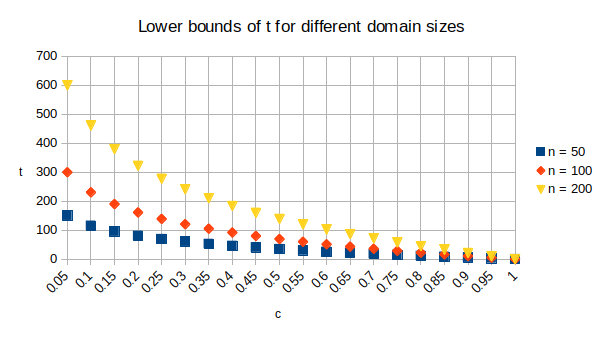
\includegraphics[width=0.95\linewidth]{figures/3-offline/graph_t_c}
\caption{The number of required test runs as a function of the probability of false positives $c$ and size of the domain $n$}
\label{fig:graph_t_c}
\end{figure}
For assertions with several quantifiers, which are translated to random generators, all domains have to be considered in the calculation. Revisiting the intersection of sets from \secref{sec:existential}, every element in set $U$ has to be compared to every element in set $V$. Thus, the lower bound of test runs needed to check whether they intersect with a certainty of 63.21\% is given by $t \leq t_1 * t_2$ with $t_1 \geq |U|$ and $t_2 \geq |V|$.

\subsection{Validators vs. test runs}
The last section derived a formula to calculate a lower bound for a number of test runs $t$ in order to reach a certain level of confidence. However, $t$ is not a parameter that can be adjusted to an arbitrary value on the blockchain, as the assertion is checked by the validators. Assuming a blockchain has $m$ validators, the actual lower bound of test runs is $m$. For cases where there are not enough validators to reach a threshold $c$, a mechanism is required to have each validator check the property for multiple random values. Hence, the actual executed number of checks is always a multiple of $m$. \secref{} goes into more detail about this based on the Tezos blockchain. \todo{Refer to section}

\subsection{Alternatives to random testing}\label{sec:alt_random}
For applications where higher reliability is crucial, an alternative to checking elements randomly could be to coordinate a systematic iteration of the domain. The implementation of such a coordination is not trivial though; validators can't simply be passed an individual value as input. Instead, possible approaches could be to implement a central instance that allocates an element in the search space to each validator, or use some unique and intrinsic attribute, like an identification number, as input for a mapping. The discussion if this approach would provide any advantages over a local validation of the property is left open \todo{Depends on cost analysis?}.

\subsubsection{Central instance assigning values}
For this approach, the tool-chain would need to generate a separate contract that is called by the miners and validators as a proxy. This contract would then, for instance, generate a number using a modulo-n counter and pass this number as an additional parameter to the assertion code. The random generators would be omitted accordingly. However, this works only as expected if there are no simultaneous transactions calling the contract, otherwise it cannot be guaranteed that all elements have been checked for each of the transactions. If and how this issue can be solved will not be discussed further in this thesis.
\todo{Serializes tests -> see expose rejected ideas}

\subsubsection{Using unique attributes of a validator}\label{sec:alt_attributes}
This approach strongly depends on whether the validators have a unique id or other attribute that can be accessed from within a contract.  If there is (or the language can be extended with such a feature), there needs to exist a non-injective surjective function that maps the respective attributes represented by type A to an element of the domain represented by type B, i.e. $f: X \rightarrow Y$. Furthermore, for cases where $t > m$, an offset needs to be added, s.t. a validator checks distinct elements for each test run. \\
Implementing such an approach on Tezos becomes even more challenging due the way endorsing (i.e. validation) rights are distributed in its proof-of-stake mechanism: for each block level, endorsing rights are assigned to the owner of a randomly selected roll, i.e., a set of tokens \cite{tezos_docs}. This means that the same validator can be picked multiple times for endorsing one block and thus some elements in the domain may remain unchecked. \secref{} goes into more detail about this issue. \todo{Ref section}